Um die Entwicklungen der Angular PWA und der nativen Swift-App zu vergleichen, wird die im Folgenden beschriebene Punktematrix verwendet. Bei der Evaluation soll auf verschiedene Aspekte der beiden Projekte eingegangen werden. Diese sind wie folgt:
\begin{description}
	\item [Anwendung]
		Die Kriterien zur Anwendung (bzw. App) beziehen sich auf die Eigenheiten der Apps, darunter die Installation, die Aktualisierung und die Plattformabhängigkeit.
		
	\item [Entwicklung]
		Kriterien der Entwicklung beziehen sich auf die Programmierung und Umsetzung der funktionalen und nicht-funktionalen Anforderungen.
		
	\item [Nutzung]
		Der Aspekt Nutzung betrachtet die Anwendung aus Nutzerperspektive.
		
\end{description}

\begin{table}[h]
	\centering
	\begin{tabularx}{\textwidth}{|l||c|c|c|c|c|c|}
		\hline
		Kriterium              & - - & - & neutral & + & ++ & Gesamtanteil \\
		\hline
		\multicolumn{7}{c}{Anwendung}                                      \\
		\hline
		Plattformabhängikeit   & 0   & 1 & 2       & 3 & 4  & 10\%         \\
		Installation           & 0   & 1 & 2       & 3 & 4  & 5\%          \\
		Speicherzugriff        & 0   & 1 & 2       & 3 & 4  & 5\%          \\
		Speicherbedarf         & 0   & 1 & 2       & 3 & 4  & 5\%          \\
		Aktualisierbarkeit     & 0   & 1 & 2       & 3 & 4  & 5\%          \\
		Konsistenz des Designs & 0   & 1 & 2       & 3 & 4  & 5\%         \\

		\hline
		\multicolumn{7}{c}{Entwicklung}                                    \\
		\hline
		Bibliotheken           & 0   & 1 & 2       & 3 & 4  & 10\%         \\
		Umsetzung              & 0   & 1 & 2       & 3 & 4  & 20\%         \\
		Testbarkeit            & 0   & 1 & 2       & 3 & 4  & 10\%         \\
		Vorausgesetzte Entwicklungserfahrung    & 0   & 1 & 2       & 3 & 4  & 10\%         \\

		\hline
		\multicolumn{7}{c}{Nutzung}                                        \\
		\hline
		Verständlichkeit       & 0   & 1 & 2       & 3 & 4  & 10\%         \\
		\hline

		\hline
		Summe                  & 0   & 1 & 2       & 3 & 4  & 100\%        \\
		\hline
	\end{tabularx}
	\caption{Punktekatalog für Kriterien} \label{tab:punktekatalog}
\end{table}

%	Plattformabhängikeit   & 0   & 1 & 2       & 3 & 4  & 10\%         \\
%Installation           & 0   & 1 & 2       & 3 & 4  & 5\%          \\
%Speicherzugriff        & 0   & 1 & 2       & 3 & 4  & 5\%          \\
%Speicherbedarf         & 0   & 1 & 2       & 3 & 4  & 5\%          \\
%Aktualisierbarkeit     & 0   & 1 & 2       & 3 & 4  & 5\%          \\
%Konsistenz des Designs & 0   & 1 & 2       & 3 & 4  & 5\%         \\
%Bibliotheken           & 0   & 1 & 2       & 3 & 4  & 10\%         \\
%Umsetzung              & 0   & 1 & 2       & 3 & 4  & 20\%         \\
%Testbarkeit            & 0   & 1 & 2       & 3 & 4  & 10\%         \\
%Vorausgesetzte Entwicklungserfahrung    & 0   & 1 & 2       & 3 & 4  & 10\%         \\
%Verständlichkeit       & 0   & 1 & 2       & 3 & 4  & 10\%         \\
%
\begin{figure}[h]

	\begin{tikzpicture}
	
		% Diagram setup
		\tkzKiviatDiagram[scale=1.0,label distance=.5cm,
		radial  = 4,
		gap     = 1,  
		lattice = 4]{
			Plattformabhängigkeit,
			Installation,
			Speicherzugriff,
			Speicherbedarf,
			Aktualisierbarkeit,
			Designs,
			Bibliotheken,
			Umsetzung,
			Testbarkeit,
			Vorausgesetzte Entwicklungserfahrung,
			Nutzerfreundlichkeit
		}
		
		% native App
		\tkzKiviatLine[thick,color=blue,mark=ball,
		fill=blue!20,opacity=.5](2,4,4,2,3,3,1,2,3,3,4)
		
		% PWA
		\tkzKiviatLine[thick,color=green,mark=ball,
		fill=green!20,opacity=.5](3,2,3,4,4,1,4,4,4,1,2)
		
		\tkzKiviatGrad[prefix=,unity=1,suffix=](0)  
	

	
	\end{tikzpicture}
	
	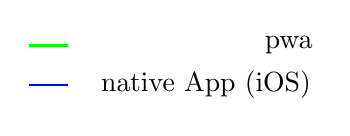
\begin{tikzpicture}
	%\draw[draw=black!20] (-0.1,-0.2) rectangle ++(15,0.5);
	
	\draw [thick, green] (0,0.5) -- (0.5,0.5); 
	\node at (3.3,0.5) {\acf{pwa}};
	
	\draw [thick, blue] (0,0) -- (0.5,0); 
	\node at (2.25,0) {native App (iOS)};
	

		\end{tikzpicture}
	
	\caption{Spinnennetzdiagram: Kriterienvergleich \acs{pwa} und native App}
\end{figure}

\textbf{Erläuterung:}
Grundsätzlich gibt es einen Punktabzug, wenn der*die Nutzer*in grundlegenden Funktionen explizit zustimmen muss. Das Idealbild ist eine sofort nutzbare Anwendung, die ohne weitere Zwischenschritte den kompletten Funktionsumfang besitzt.
\begin{description}
	\item [Plattformabhängigkeit]
	      Wie viele Plattformen beziehungsweise Betriebssysteme werden unterstützt?
	      Ist die Nutzung auf Smartphone begrenzt oder kann die Anwendung auch auf einem Tablet oder Desktop installiert werden?

	\item [Installation]
	      Die App sollte ohne mehrere Zwischenschritte nutzbar sein. Ist die Installation zu kompliziert, führt dies zu Punktabzug.

	      Es fließt mit ein, wie viel Aufwand betrieben werden muss, um die App einem Publikum zur Verfügung zu stellen. Dieser Aufwand ist idealerweise gering und im Interesse des*der Entwicklers*in.

	\item [Speicherzugriff]
	      Anwendungen müssen Daten speichern können, um dem Nutzer einen Mehrwert zu bieten. Die Größe der zu speichernden Daten ist bei diesem Vergleich auf Kilobyte zu begrenzt. Gibt es die Möglichkeit Dateien abzulegen ist dies positiv zu werten.
	      Können Daten nur temporär und nicht persistent gespeichert werden, führt dies zu starkem Punktabzug. Idealerweise können Daten in gängigen Formaten (beispielsweise JSON, CSV, XML oder Plaintext) gespeichert werden. Muss der*die Nutzer*in dem Speichern von Daten aktiv zustimmen, stört dies die Nutzungserfahrung und ist daher negativ zu werten.

	\item [Speicherbedarf]
	      Der Speicherplatz eine Smartphones ist deutlich kleiner, als der eines Desktop-Computers. Bestenfalls ist die Anwendung nur wenige Megabyte groß und kann so schnell über eine mobile Datenverbindung installiert und upgedated werden.
	      Hoher Speicherverbrauch führt zu Punktabzug, wohingegen geringer Speicherverbrauch positiv bewertet wird. Der Verbrauch ist unter den einzelnen Plattformen relativ zu bewerten.

	\item [Aktualisierbarkeit]
	      Idealerweise kann die Installation von Updates vom Entwickler*in kontrolliert werden. Schnelle Updatezyklen sind wünschenswert, da in der Praxis dadurch schnell Sicherheitslücken und Bugs behoben werden können. Wenn ein Nutzer sich aktiv gegen Updates weigern kann, oder diese manuell installieren muss könnte dies zu Kompatibilitätsproblemen mit Webschnittstellen oder Sicherheitsproblemen führen und führt deshalb zu Punktabzug.

	      Der Aufwand der betrieben werden muss, um Updates einzubringen wird mitevaluiert. Je schneller Updates flächendeckend auf den Geräten der Nutzer*innen landen, desto höher die Punktzahl.

	\item [Konsistenz des Designs]
	      Idealerweise sieht die Anwendung auf verschiedenen Geräten identisch aus. Grundsätzlich wird erwartet, dass Schriften, Farben und Größenverhältnisse auf unterschiedlichen Geräten und gegebenenfalls unterschiedlichen Browsern ein konsistentes Bild ergeben.
	      Eine skalierende Nutzeroberfläche ist wünschenswert. Anzeigefehler, wie beispielsweise überlappende Objekte, fehlerhafte Elemente oder fehlende Schriftarten führen zu Punktabzug. Auch der Aufwand welcher betrieben werden muss, um das Nutzerinterface skalierbar zu gestalten fließt in die Bewertung mit ein.

	\item[Verständlichkeit für den*die Nutzer*in]
	      Dem*der Nutzer*in sollte zu jedem Zeitpunkt klar sein, wie die Anwendung installiert, gestartet und deinstalliert werden kann. Ist dies nicht gewährleistet werden Punkte abgezogen.

	\item[Bibliotheken]
		Für die Entwicklung wird angenommen, dass die Möglichkeit, Bibliotheken für die Programmierung zu nutzen, wertgeschätzt wird. Aufgrund praktischer Erfahrungen wird angenommen, dass diese (richtig eingesetzt), den Programmieraufwand oft reduzieren. In der Evaluierung werden Bibliotheken von open-source Organisationen und gegebenenfalls Bibliotheken des Plattformanbieters (Apple, Google, Mozilla etc.) betrachtet. In die Bewertung fließt ein, wie einfach ein*e Entwickler*in diese Bibliotheken nutzen und gegebenenfalls installieren kann. 

	\item[Umsetzung]
		
	\item[Testbarkeit]
	
	\item[Vorausgesetzte Entwicklungserfahrung]
		Es soll eingeschätzt werden, wie hoch die Einstiegshürde für die Entwicklung der jeweiligen Technologie ist. Die Anzahl und Komplexität der Tools fließt in die Bewertung mit ein. Es wird an genommen, dass die Entwicklung mit einem einzigen Werkzeug für den*die Entwickler*in einfacher ist, als das Bedienen mehrerer komplexerer Entwicklungstools. Gibt es grafische Oberflächen für viele Entwicklungsschritte ist dies positiver zu bewerten, als das Arbeiten mit Skripten und der Kommandozeile.
		
\end{description}

